\chapter{嵌入式硬件平台简介及内核运行}
\section{基于嵌入式硬件的操作系统开发流程}

\subsection{串口简介}

\subsubsection{什么是串口}

串口是串行接口(Serial Port)的简称,是一种常用的计算机接口。由于连线少、通信控制简单而得到广泛的使用。串口有几种标准,常见的一种称为 RS232 接口的标准是在1970年由美国电子工业协会(EIA)和几家计算机厂商共同制定的。RS232标准应用广泛,其全称是“数据终端设备(DTE)和数据通讯设备(DCE)串行二进制数据交换接口”,该标准定义了串口的电气接口特性和各种信号电平等。


标准串口协议支持的最高数据传输率是115Kbps。一些改进的串口控制器支持更高甚至460Kbps的数据传输率,如增强型串口ESP(Enhanced Serial Port)和超级增强型串口Super ESP。


RS232 串口使用D型数据接口,最初有9针和25针两种连接方式。随着计算机技术的不断进步,25针的串口连接方式已经被淘汰,目前所有的RS232串口都使用9针连接方式。

\subsubsection{串口工作原理}

串口通过直接连接在两台设备之间的线发送和接收数据,两台设备通信最少需要三根线(发送数据、接收数据和接地)才可以通信。以最常见的RS232串口为例,通信距离较近时(<12m),可以用电缆线直接连接标准RS232端口。如果传输距离远,可以通过调制解调器(MODEM)传输。因为串口设备工作频率低且容易受到干扰,远距离传输会造成数据丢失。

\begin{table}[!ht]
	\centering
	\begin{tabular}{|c|c|c|}
		\hline
		\textbf{针号} & \textbf{功能说明} & \textbf{缩写} \\
		\hline
		1 & 数据载波检测 & DCD  \\
		2 & 接收数据 & RXD  \\
		3 & 发送数据 & TXD \\
		4 & 数据终端准备 & DTR \\
		5 & 信号地 & GND \\
		6 & 数据设备准备好 & DSR \\
		7 & 请求发送 & RTS \\
		8 & 清除发送 & CTS \\
		9 & 振铃指示 & BELL \\
		\hline
	\end{tabular}
	\caption{DB9接口的RS232 串口数据线定义}
	\label{DB9接口的RS232 串口数据线定义}
\end{table}

表 \ref{DB9接口的RS232 串口数据线定义}是常见的9针接口串口各条线定义,RS232标准的串口不仅提供了数据发送和接收的功能,同时可以进行数据流控制。对于普通应用来说,连接好两个数据线和地线就可以通信。

\subsubsection{Windows系统下的串口工具}

MobaXterm 又名 MobaXVT,是一款增强型终端、X 服务器和 Unix 命令集(GNU/ Cygwin)工具箱。可以开启多个终端视窗,以最新的 X 服务器为基础的 X.Org,可以轻松地来试用 Unix/Linux 上的 GNU Unix 命令。这样一来,我们可以不用安装虚拟机来试用虚拟环境,然后只要通过 MobaXterm 就可以使用大多数的 linux 命令。MobaXterm 还有很强的扩展能力,可以集成插件来运行 Emacs、Fontforge、Gcc, G++ and development tools、MPlayer、Perl、Curl、Corkscrew、 Tcl / Tk / Expect、 Screen、 Png2Ico 、 NEdit  Midnight Commander 等程序。


MobaXterm的下载较为简单,进入官网直接下载即可。需要注意的是MobaXterm 分免费家庭版和收费专业版:
\begin{itemize}
	\item 家庭版(Home):家庭版又分便捷版和安装版。便捷版不需要安装,下载压缩包后解压即可使用。安装版则需一步步安装后才能使用。
	\item 专业版(Professional):专业版会在 Session数、SSH tunnels 数和其他一些定制化配置进行限制。
\end{itemize}

MobaXterm的界面结构为:
\begin{itemize}
	\item 主页:打开MobaXterm后,绝大部分内容会被主页占据,主页有快捷按钮“start local terminal”以及最近的Session记录,可以方便打开终端,进行命令行操作。
	\item 菜单栏:MobaXterm的菜单栏如下,分为menu bar和buttons bar两行。用户可通过menu bar设置MobaXterm。buttons bar则为用户提供了一系列功能,如用户可通过Session启动远程会话,选择创建 SSH、Telnet、Rlogin、RDP、VNC、XDMCP、FTP、SFTP 或串行会话。开始的每个会话都会自动保存并显示在左侧边栏中。
	\item 侧边栏:侧边栏分为三个视图,分别为Sessions,Tools,Macros。Sessions负责管理使用过的Session配置,可以在任意Session选项上右击进行编辑。Tools分为四部分Terminal games、System、Office、NetWork的工具集合。使用非常的方便。Macros可以录制操作过程,下次使用时直接回放即可。
\end{itemize}

\begin{figure}[h]
	\centering
	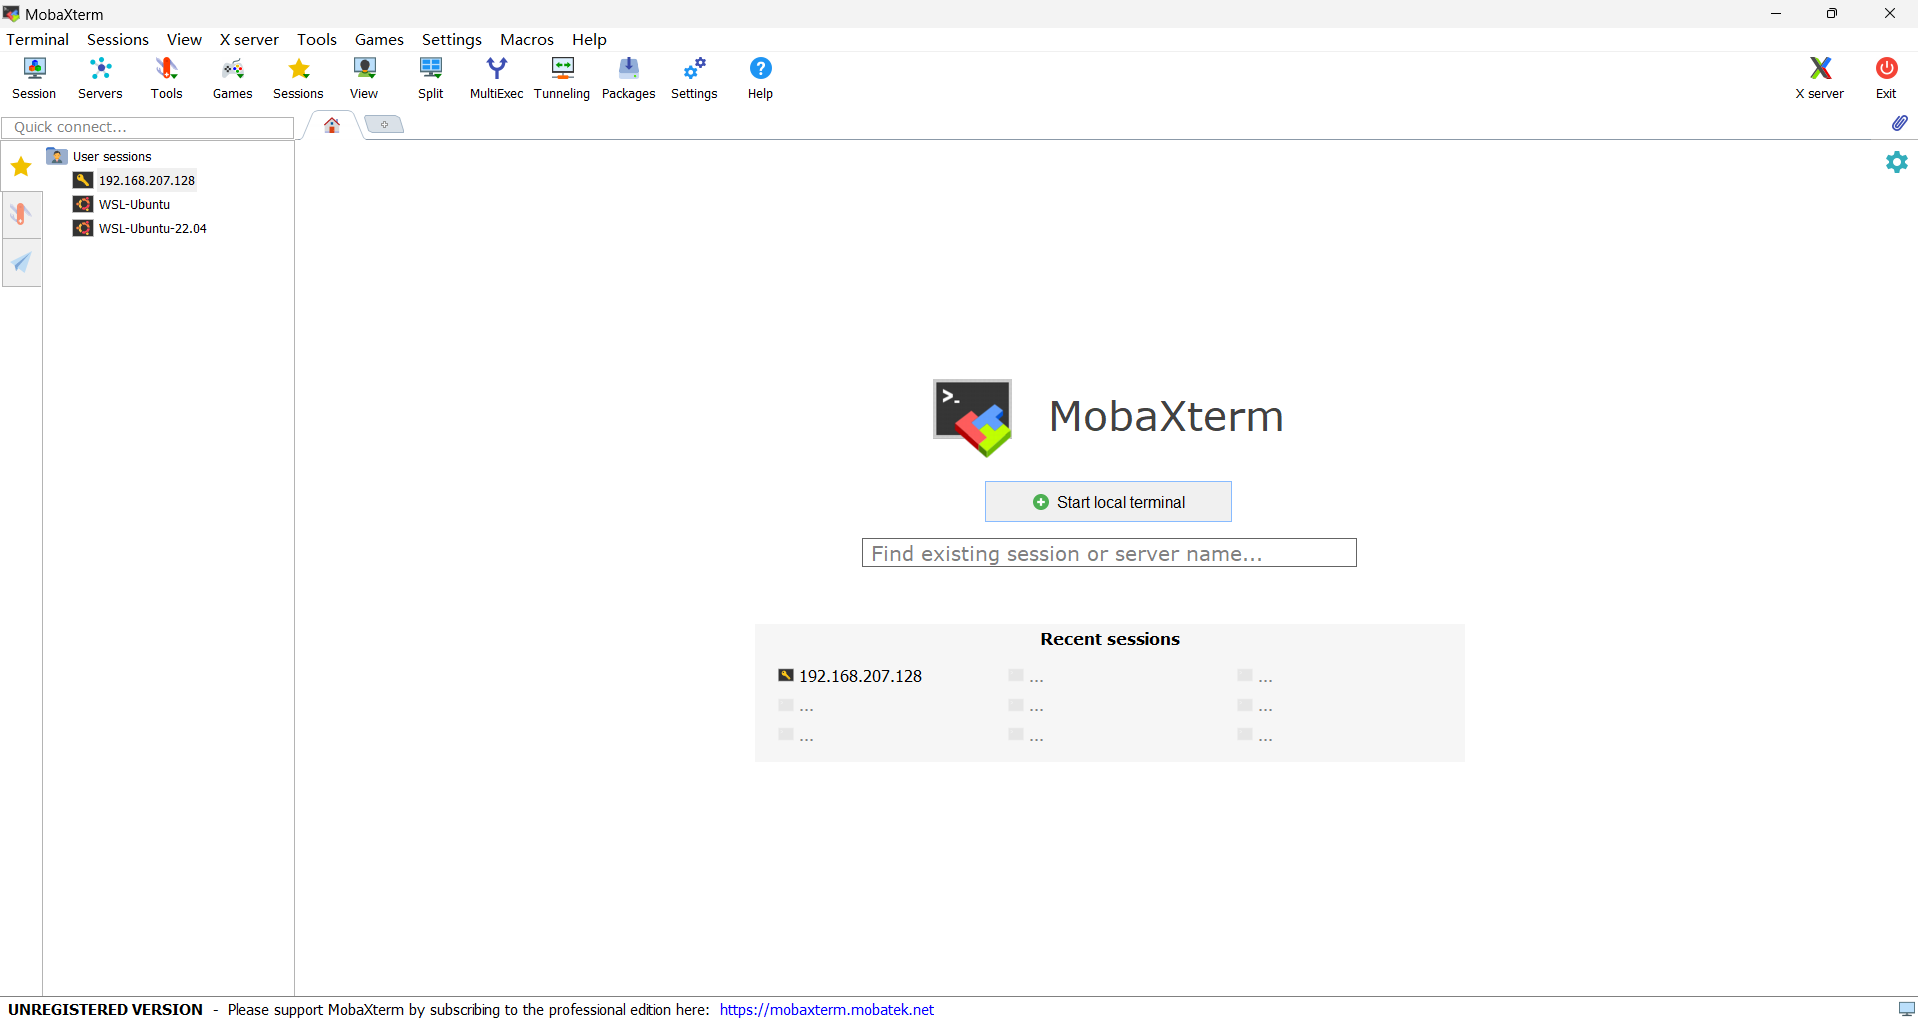
\includegraphics[width=0.6\textwidth]{figures/08-01-mobaXterm界面.png}
	\caption{mobaXterm界面}
	\label{mobaXterm界面}
\end{figure}


MobaXterm是一款功能强大的综合性工具,支持SSH、RDP、FTP、Serial等多种通信协议。在本节中,我们将重点介绍其支持的Serial协议功能。MobaXterm可用作串口终端,与串口调试助手等工具相比,它提供了更强大的功能。在使用串口调试助手等工具时,虽然可以用于打印调试信息,但无法实现终端使用,即不能输入命令。


在MobaXterm中,通过点击"Session",选择"Serial",打开串口设置窗口。首先,选择要配置的串口号,并使用串口线将开发板连接到计算机上。然后,设置波特率,MobaXterm软件能够自动识别串口,用户只需从下拉菜单中选择相应的波特率。此外,还需进行其他串口功能的设置。点击"Advanced Serial settings"选项卡,可配置串口的其他功能,包括串口号、数据位、停止位、奇偶校验和硬件流控等。若需配置与终端相关的功能,则可点击"Terminal settings",进行相关设置,如终端字体以及字体大小等。完成设置后,点击窗口下方的"OK"按钮即可。

\subsubsection{Linux系统下的串口工具}

串口是嵌入式开发使用最多的通信方式。Linux系统提供了一个串口工具minicom,可以完成复杂的串口通信工作。若将minicom移植到板卡上,我们就可以借助minicom对串口进行读写操作。


本节介绍 minicom的使用。首先是安装 minicom,在 Ubuntu Linux 系统 shell 下输入“sudo apt-get install minicom”,按回车键后即可安装minicom 软件。软件安装好后,第一次使用之前需要配置minicom。

\begin{enumerate}
	\item 在shell中输入 sudo minicom-s,出现 minicom配置界面,下图 \ref{minicom配置界面}所示。minicom配置菜单在屏幕中央,每个菜单项都包括了一组配置。
	\begin{figure}[h]
		\centering
		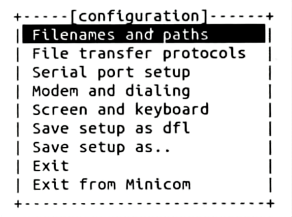
\includegraphics[width=0.4\textwidth]{figures/08-01-minicom配置界面.png}
		\caption{minicom配置界面}
		\label{minicom配置界面}
	\end{figure}

	\item 用光标键移动高亮条到 Serial Port setup菜单项,按回车键后进入串口参数配置界面,如下图 \ref{minicom配置端口界面}所示。串口配置界面列出了串口的配置,每个配置前都有一个英文字母,代表进入配置项的快捷键。首先配置端口,输入小写字母a,光标移动到了/dev/tty8字符串最后,并且进入
	到编辑模式。以笔者机器为例,修改为/dev/tty0,代表连接到系统的第一个串口。
	\begin{figure}[h]
		\centering
		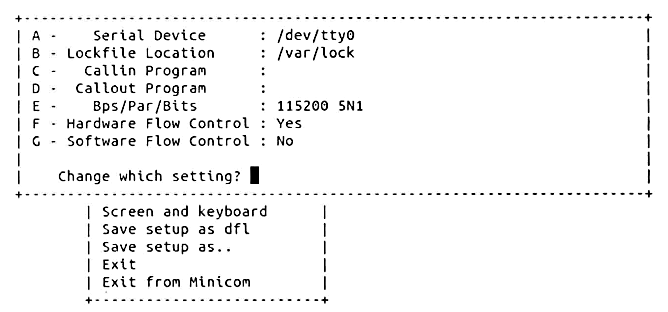
\includegraphics[width=0.6\textwidth]{figures/08-01-minicom配置端口界面.png}
		\caption{minicom配置端口界面}
		\label{minicom配置端口界面}
	\end{figure}

	\item 配置好串口设备后按回车键,保存参数并且回到提示界面。输入小写字母e,进入串口参数配置界面,如下图 \ref{minicom配置串口参数}所示。串口参数界面可以配置串口波特率、数据位、停止位等信息。一般只需要配置波特率,如在笔者机器上需要配置波特率是38400,输入小写字母d,屏幕上方current字符串后的波特率改变为38400。
	\begin{figure}[h]
		\centering
		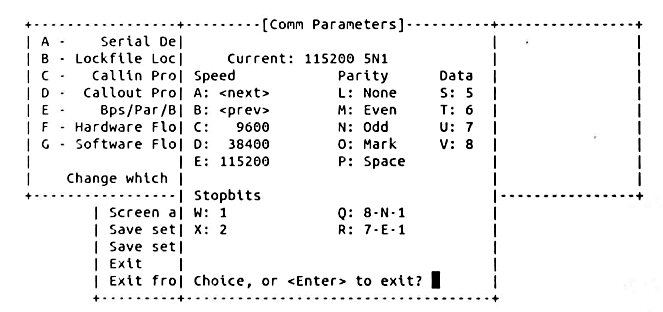
\includegraphics[width=0.6\textwidth]{figures/08-01-minicom配置串口参数.png}
		\caption{minicom配置串口参数}
		\label{minicom配置串口参数}
	\end{figure}

	\item 设置好波特率后按回车键,保存退出,回到串口配置界面,如下图 \ref{minicom配置端口结束}所示。串口被设置为tty0,波特率是38400,其他配置使用默认设置。如果保存配置,直接按回车键退出。选择Save setup as dfl选项后按回车键,配置信息被保存为默认配置文件,下次启动的时候会自动加载。保存默认配置后,选择Exit选项后按回车键,退出配置界面,minicom自动进入终端界面。在终端界面会自动连接到串口,如果串口没有连接任何设备,屏幕右下角的状态提示为Offline。
	\begin{figure}[h]
		\centering
		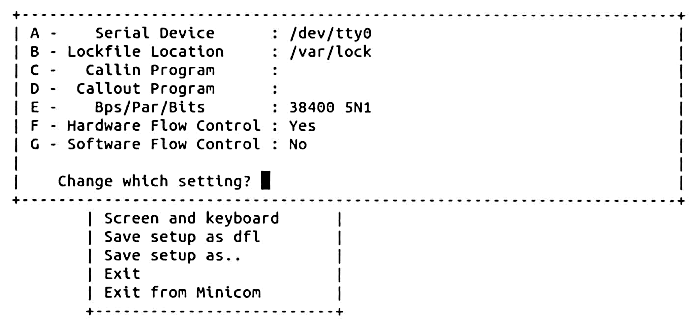
\includegraphics[width=0.6\textwidth]{figures/08-01-minicom配置端口结束.png}
		\caption{minicom配置端口结束}
		\label{minicom配置端口结束}
	\end{figure}

	\item 退出 minicom,使用Ctrl+a键,然后输入字母z,出现minicom的命令菜单,如下图 \ref{minicom命令界面}所示。
	\begin{figure}[h]
		\centering
		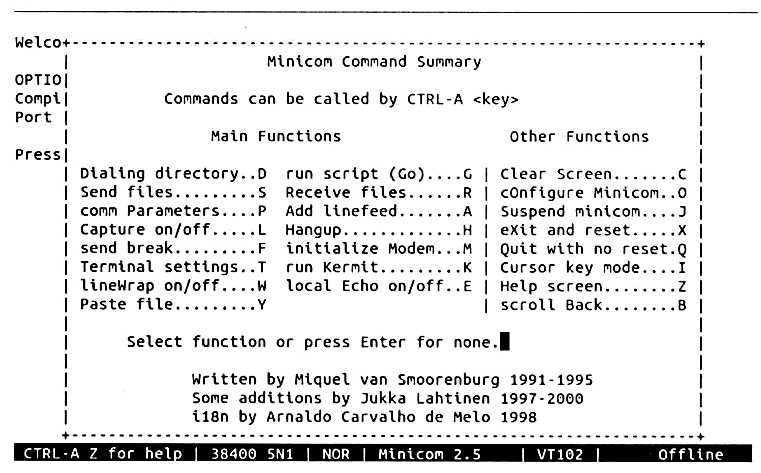
\includegraphics[width=0.6\textwidth]{figures/08-01-minicom命令界面.png}
		\caption{minicom命令界面}
		\label{minicom命令界面}
	\end{figure}
\end{enumerate}



Minicom 提供了丰富的功能,是 Linux 中串口通信和远程管理的重要工具:

\begin{itemize}
	\item 调试和配置串口设备: Minicom 可以连接和调试各种串口设备,如调制解调器、路由器、交换机等。用户可以通过 Minicom 查看设备的输出信息,发送指令进行配置和调试。

	\item 远程终端连接: Minicom 可以作为一个终端仿真器,用于远程连接到其他计算机或设备。通过串口连接,用户可以在本地计算机上操作远程设备,进行远程管理和维护。

	\item 数据传输和文件传输: Minicom 支持通过串口进行数据传输,可用于传输文件、备份数据等。用户可以通过 Minicom 将文件发送到远程设备或从远程设备接收文件。

	\item 系统调试和故障排查: Minicom 可用于调试和排查系统故障。通过串口连接到系统控制台,用户可以查看系统的启动信息、错误日志等,帮助定位和解决问题。

	\item 嵌入式开发和调试: 对于嵌入式系统开发者来说,Minicom 是一个重要的工具。它可用于与嵌入式设备进行通信,进行程序下载、调试和测试。
\end{itemize}